\documentclass[10pt,twocolumn]{article}

\input{style}
\title{TSBB08 \\ Segmentation of cells in microscopy images}
\author{Alexander Poole \\ Anna Hjelmberg}


%%Dokumentets början
\begin{document}
\maketitle
	\thispagestyle{empty}
\newpage

\section{Summary}
The goal of this laboration rapport is to show how one can segment cells in an
microscopy images and then locate and count padlock-signals in each cell.
The methods described in this rapport can be used on any microscopy image of decent quality.
But in this rapport we have primarily been working with image \ref{fig:ImColour},
which when divided into looks like image \ref{fig:CellLinesNCircles}.
In image \ref{fig:CellPart} we have isolated a single cell and counted its 14 padlock signals.

\begin{figure}[ht]
\centering
\includegraphics[width=0.3\textwidth]{Bilder/ImColour.pdf}
\caption{The original image.}
\label{fig:ImColour}
\end{figure}

\begin{figure}[ht]
\centering
\includegraphics[width=0.3\textwidth]{Bilder/CellLinesNCircles.pdf}
\caption{The original image where cells have been segmented and padlock signals in cell nr 6 have been marked.}
\label{fig:CellLinesNCircles}
\end{figure}

\begin{figure}[ht]
\centering
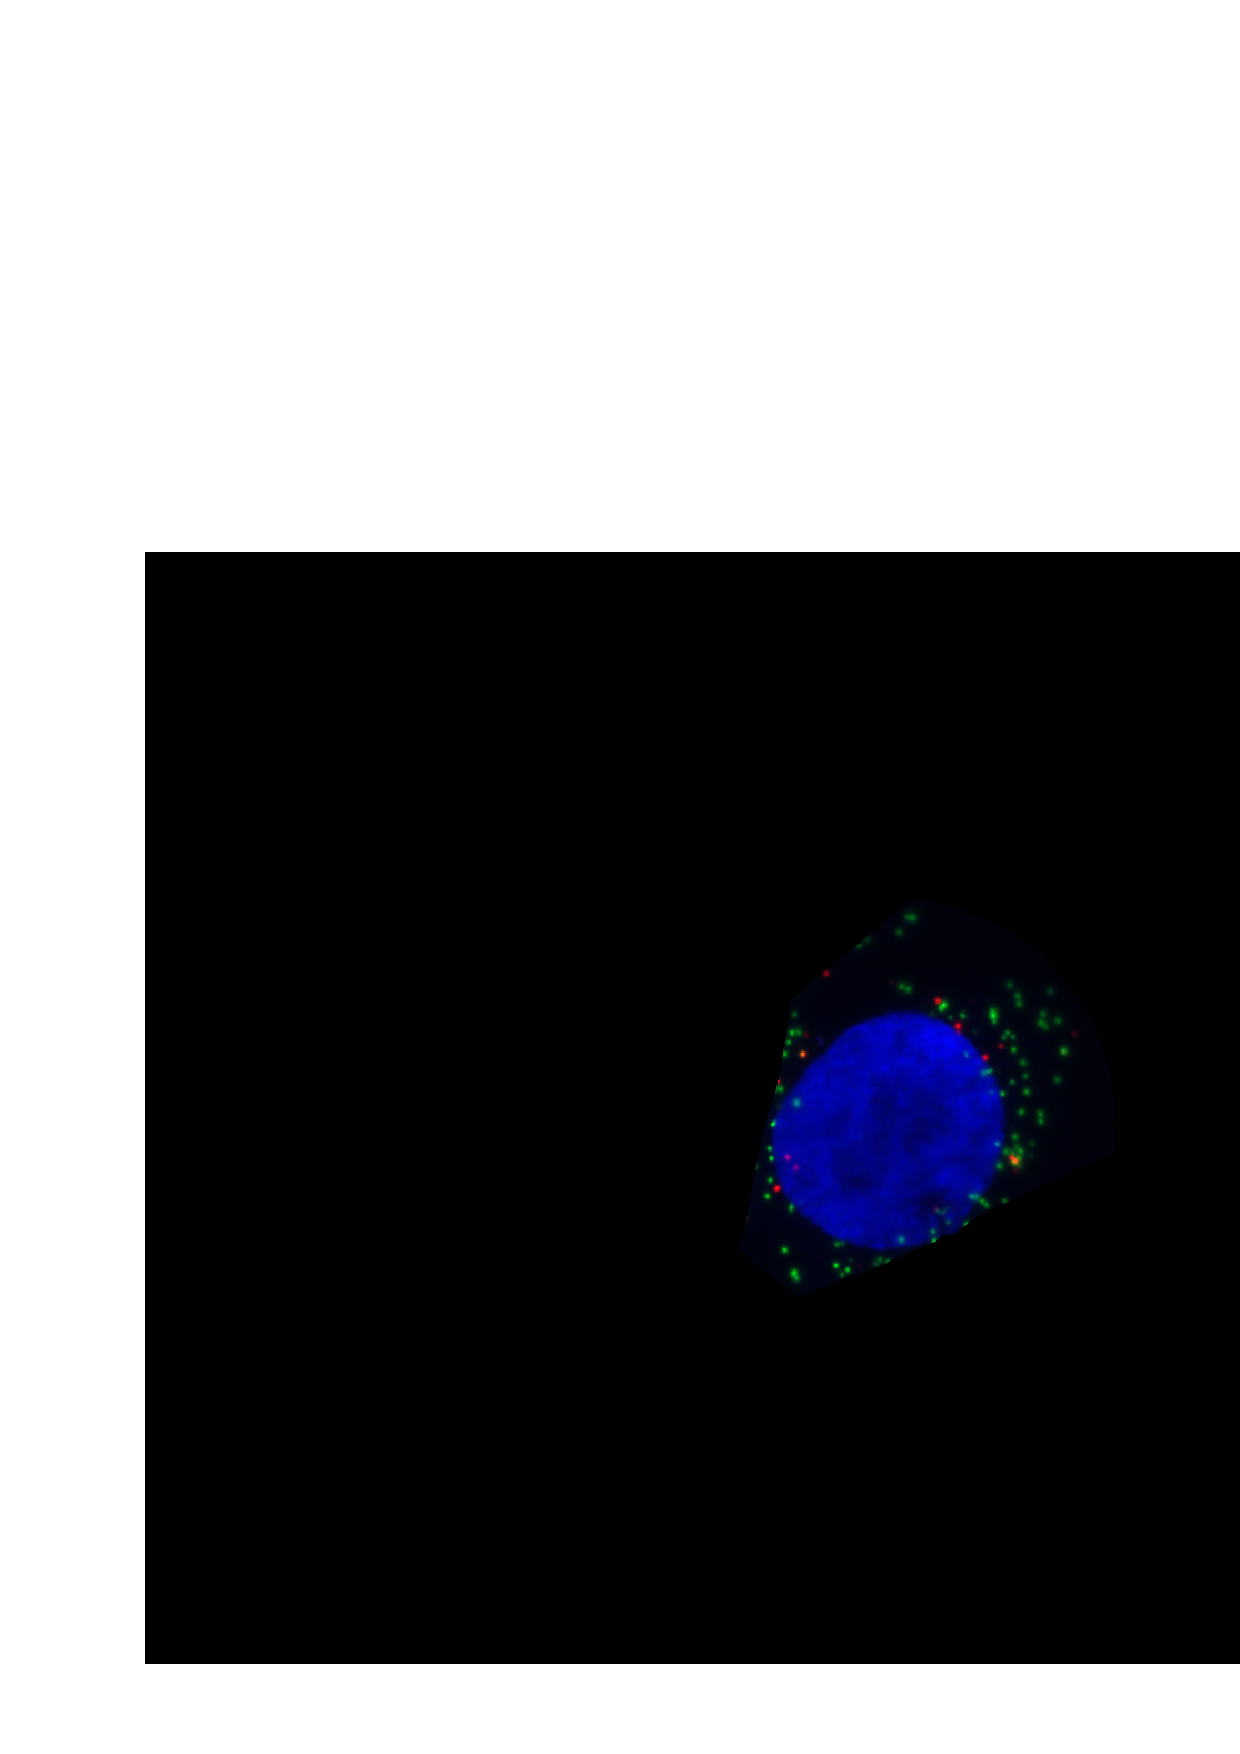
\includegraphics[width=0.3\textwidth]{Bilder/CellPart.pdf}
\caption{Cell nr 6 taken out of the original image.}
\label{fig:CellPart}
\end{figure}


To get the image shown in image \ref{fig:CellLinesNCircles} segmentation
on the original image has to be done. To do so the first step is to get an "clean" image over the
six cell kernels. This is done by threshholding image 4 (!!!!!!!INSERT IMAGE 4!!!!!!) which is
just the blue part of the original image. The threshhold is determined by looking at
a histogram of the blue original image. When the image is threshholded it still
contains some rubbish, see image 6 (!!!!!!!!!!INSERT IMAGE 6!!!!!!!).
By performing opening and closing the rubbish is removed from the image and image 7
	(!!!!!!!!!INSERT IMAGE 7!!!!!!!) is reseved.

When a clean image over the cell kernels is made a watershed algorithm is performed
on the image. First a distance transform is made inside the objects and then the sign
of the distance transform is changed and the pixels outside the objects are set
to the minimum value, see image 13 and image 10
(!!!!INSERT IMAGE 13!!!!)(INSERT IMAGE 10). All of the regional minimum values
are located and labeled. Image 11 (!!!!!INSERT IMAGE 11!!!!!!!!!!!) is a close up
on some of the regional minimums that are found. The purpose of finding the
regional minimum values is to get one minumum value in each cell kernel so that
the watershed transform algorithm can be executed. As shown in image 11 there are
more then one minimum value in each kernel and also some "false minimum" inbetween
the two kernels that is overlapping. To get rid of these "false minimum values" a
demand on the depth of the minimum values are set. This removes some of the unwanted
minimums but there are still some extra minimums in the middle of the kernels. This
was solved by performing opening on the image which made the close single pixel
minimums into one minimum containing several pixels, see image 14 (!!!!!INSERT A ZOOMED IN IMGE 14!!!).




\section{Watershed segmentation 1}
Inorder to use our warershed algorithm we first need to get a binnary image of the cell kernels. The cell kernels are mostly located
in the blue image so we start by looking at it's hitogram and then threshholding it. That gives us

\section{Watershed segmentation 2}

\section{Morphological image processing}

\section{Localization of padlock-signals}


\end{document}
